\chapter{Evaluation}\label{chap:evaluation}
Through the use of the framework described in the previous chapter, we evaluate four different algorithms for next-activity prediction: Two implementations that mimic Evermann et al. and Schönig et al, and the previously presented PFS and SP2. In doing so, we will analyze the different approaches for structuring the training data for performance differences.

As we follow the KDD process, this chapter briefly leads through the data processing and transformation phases in \autoref{sec:eval:data-preprocessing} and \autoref{sec:eval:data-transformation}. The latter section also covers the strategy used to engineer the SP-2 and subsequence features. Then, the test setup and the used training strategy is presented in \autoref{sec:eval:test-setup}, followed by the set of criteria by which we judge the results in \autoref{sec:eval:criteria}. Finally, the chapter ends with the presentation and discussion of the results in \autoref{sec:eval:results}. Used and relevant technologies are highlighted in the respective sections.

\section{Data preprocessing}
\label{sec:eval:data-preprocessing}
In the first step of the KDD process~\cite{fayyad1996data}, the data is preprocessed to eliminate generally known properties that hinder machine learning model performance. In our case, this encompassed two steps for both BPIC2011 and BPIC2017 datasets:

\begin{enumerate}
    \item All columns which exhibited zero entropy, i.e. which contained a single value, were dropped.
    \item Features which correlated strongly were eliminated. To account for categorical correlation, the bias-corrected version of Cramér's~V~\cite{bergsma2013bias} was used.
\end{enumerate}

\todo[inline]{adapt to bpic2017}
In step 1, one column was dropped in BPIC2011 and two were dropped in BPIC2017.
In step 2, the bi-directional results in \autoref{fig:bpic2011-correlation-heatmap} from Cramér's V revealed that the variables \texttt{Producer code}, \texttt{Activity code} and \texttt{Specialism code} correlate strongly with many others in the BPIC2011 dataset. Thus, these were dropped. As evidenced in \autoref{fig:bpic2012-correlation-heatmap}, the BPIC2017 dataset with its small number of features did not require any removals.

\begin{figure}
\centering
\subfloat[][BPIC2011 Cramér's V heatmap]{
    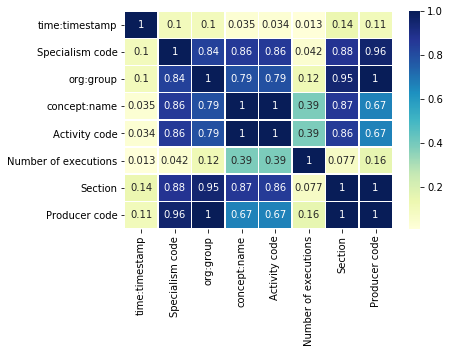
\includegraphics[width=0.7\textwidth]{gfx/bpic2011-correlation-matrix.png}
    \label{fig:bpic2011-correlation-heatmap}
}
\qquad
\subfloat[][BPIC2012 Cramér's V heatmap]{
    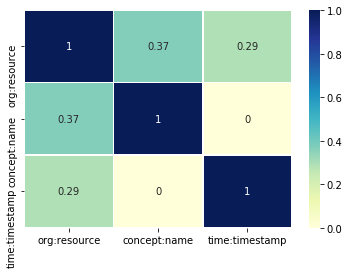
\includegraphics[width=0.7\textwidth]{gfx/bpic2012-correlation-matrix.png}
    \label{fig:bpic2012-correlation-heatmap}
}
\caption{Correlation heatmaps obtained from Cramér's~V.}
\end{figure}

The activities described above were conducted in JupyterLab notebooks~\cite{web:jupyter}, where Anaconda~\cite{web:anaconda} was used to create a stable development environment. The OpyenXes~\cite{web:opyenxes} library proved to be especially useful for parsing the raw XES logs from BPIC.

\section{Data transformation}
\label{sec:eval:data-transformation}
Having removed unneeded features, the remaining ones were encoded following standard practice. Each numerical feature $x$ was normalized with values specific to each trace using the min-max method:

$$normalize(x) = \frac{x-min(x)}{max(x)-min(x)}$$

Categorical features without ordinal properties, which were all of them, were encoded using one-hot encoding if possible. In the case of the input for the Evermann model, they were encoded with dictionary encoding, as this is required for Embedding layers.

\subsection*{SP-2 feature engineering}
For every trace, SP-2 features mark whether an activity has occured yet. Thus, these features are engineered in an iterative fashion, as \autoref{lst:sp2-generation} outlines. For every trace, a new data frame \texttt{sp2\_df} is created and the occurence of the first activity is marked inside it. For all following activities, the contents of the previous row inside \texttt{sp2\_df} are copied into the current one and the presence of the current activity is marked. This repeats itself until the trace has been processed completely.

\begin{figure}
\begin{minted}{python}
sp2_df = pd.DataFrame(columns=activity_labels,
                      index=range(0,len(t)),
                      dtype=np.bool)
for col in sp2_df.columns: sp2_df[col].values[:] = 0

# mark first occuring SP-2 
cname = "{0}{1}".format(sp2_prefix, t[target_col][0])
sp2_df[cname].values[0]  = 1

for i in range(1,len(t)):
first_activity_name = t["concept:name"].iloc[i]
col = "{0}{1}".format(sp2_prefix,first_activity_name)

sp2_df.values[i] = sp2_df.values[i-1]
sp2_df[col].values[i] = 1
\end{minted}
\caption{Generating SP-2 features for a single trace \texttt{t} and a specific target column \texttt{target\_col}.}
\label{lst:sp2-generation}
\end{figure}

\subsection*{Sub-sequence feature engineering}
The sub-sequence features for the PFS model were created with the help of the \textit{prefixspan-py} library~\cite{web:prefixspan-py}. As \autoref{lst:pfs-mining} shows, the library greatly facilitates obtaining closed sequences ranked by support and returns a two-dimensional array of sub-sequences, containing one array per sub-sequence. The sequences are mined from the entirety of traces.

\begin{figure}
\begin{minted}{python}
prefixspan_traces = PrefixSpan(encoded_traces)
closed_sequences = prefixspan_traces.topk(25, closed=True)
\end{minted}
\caption{Obtaining closed sequences using the \textit{prefixspan-py} library.}
\label{lst:pfs-mining}
\end{figure}

After mining the sequences, a loop is executed for every trace, shown in \autoref{lst:subsequence-feature-creation}. For each index \verb=i= it is checked whether any of the mined subsequences starts at that position. This is checked by peeking ahead of \verb=i= for the length of the subsequence. As in the case of the SP-2 features, the occurence of a subsequence is marked with a boolean flag from the row that it occured in onwards.

\begin{figure}
\begin{minted}{python}
subseq_df = pd.DataFrame(columns=subseq_labels,
                         index=range(0,len(t)),
                         dtype=np.bool)
subseq_df[:].values[:] = False
activity_codes = t[target_col].map(event_to_int)
tlen = len(t)

for i in range(0, tlen):
  # loop through all subsequences
  for subseq_idx, subseq in enumerate(ps):
    if tlen <= i+len(subseq): continue
            
    # check if subseq takes place in the following steps
    subsequence_found = True
    j = 0
    
    while subsequence_found and j < len(subseq):
      if subseq[j] != activity_codes[j+i]:
        subsequence_found = False
        j += 1

    # if subseq took place, subsequence_found is still true
    if subsequence_found:
      subseq_df.values[j+i:,subseq_idx] = True
\end{minted}
\caption{Enriching a trace \texttt{t} with sub-sequence features by detecting those that are contained inside it.}
\label{lst:subsequence-feature-creation}
\end{figure}

\section{Test setup}
\label{sec:eval:test-setup}
To conduct the experiments, Docker containers were built with the same Anaconda environment that was used for development inside them~\cite{web:docker}. Using a version of Docker for GPU applications running on NVIDIA hardware~\cite{web:nvidia-docker}, each network-formatting combination was trained and evaluated on a single NVIDIA K80 GPU of the HPI FutureSOC Lab~\cite{web:fsoc}. The complete source code used in this thesis is available on GitHub at \href{https://github.com/flxw/master-thesis-code}{flxw/master-thesis-code}.\\

Both datasets were split into training and test sets of complete traces. While $25\%$ of the traces were used for validation and testing, the remaining $75\%$ were used for training purposes. The sets were shuffled and stratified to contain an approximately similar number of equal-length traces.

Each model implementation was trained successively with each data formatting variant on a single GPU. A model was saved when its validation loss hit a new record low. If the validation loss did not change for 10 epochs, the training was interrupted, also referred to as early stopping. \autoref{tab:network-info} illustrates information about the training setup of the networks side-by-side. As Evermann et al. made use of a version of Tensorflow that is deprecated by now, our implementation in Keras can only be understood as an approximation. Their "unrolled LSTM" can not be implemented in the same way in Keras.

\begin{table}[ht!]
    \centering
    \begin{tabular}{lcccc}
        \textbf{Network} & \textbf{Evermann} & \textbf{Schönig} & \textbf{SP2} & \textbf{PFS}\\
        \hline
        \textbf{Optimizer} & SGD\footnote{SGD stands for Stochastic Gradient Descent. Additionally setting the learning rate decay to $0.75$ at the $25^{th}$ epoch.} & RMSprop  & RMSprop & RMSprop\\
        \textbf{Loss}    &\multicolumn{4}{c}{Categorical crossentropy}\\
        \textbf{Epochs}  & 50 & 100 & 150 & 150\\
        \textbf{BPIC2011 features} & 1 & 655 & 655 + 625 & 655 + 25 \\
        \textbf{BPIC2017 features} & 1 & X & X + X & X + X \\
    \end{tabular}
    \caption{Used hyper-parameters for each model, the left two columns as chosen by the authors. The number of epochs is to be understood as the maximum number of epochs, as training may stop early.}
    \label{tab:network-info}
\end{table}

\section{Evaluation criteria}
\label{sec:eval:criteria}
The following three metrics are the focus in the evaluation of the sixteen model-formatting combinations:

\begin{enumerate}
    \item\textbf{Accuracy} - The share of correct next-activity predictions.
    \item\textbf{Resource consumption} - The amount of time and memory required during training.
    \item\textbf{Stability} - Whether the prediction accuracy begins to change as the trace progresses~\cite{francescomarino2015}.
\end{enumerate}

While the first two criteria target the usability of the results, the last one permits making a judgment about the stability of the predictions. This allows better insights into how prediction accuracy develops over time, and facilitates building trust in the model, as indicated in the introduction of the thesis.

\section{Results}\label{sec:eval:results}


\subsection*{Accuracy}
\begin{table}
\centering
\begin{tabular}{l|cccc}
    Training data format & Evermann & Schönig & SP2 & PFS\\
    \hline
    Individual &&&\\
    Grouped &&&\\
    Padded &&&\\
    Windowed &&&\\
\end{tabular}
\caption{Caption}
\label{tab:accuracy_bpic2011}
\end{table}
\begin{table}
\centering
\begin{tabular}{l|cccc}
    Training data format & Evermann & Schönig & SP2 & PFS\\
    \hline
    Individual &&&\\
    Grouped &&&\\
    Padded &&&\\
    Windowed &&&\\
\end{tabular}
\caption{Caption}
\label{tab:accuracy_bpic2017}
\end{table}

\subsection*{Resource consumption}
\begin{table}
    \centering
    \begin{tabular}{l|cccc}
        Training data format & Evermann & Schönig & SP2 & PFS\\
        \hline
        Individual &&&\\
        Grouped &&&\\
        Padded &&&\\
        Windowed &&&\\
    \end{tabular}
    \caption{Caption}
    \label{tab:resources_bpic2011}
\end{table}

\begin{table}
    \centering
    \begin{tabular}{l|cccc}
        Training data format & Evermann & Schönig & SP2 & PFS\\
        \hline
        Individual &&&\\
        Grouped &&&\\
        Padded &&&\\
        Windowed &&&\\
    \end{tabular}
    \caption{Caption}
    \label{tab:resources_bpic2017}
\end{table}

\subsection*{Stability}
\begin{figure}
    \centering
    \includegraphics{}
    \caption{Caption}
    \label{fig:earliness_bpic2011}
\end{figure}

\begin{figure}
    \centering
    \includegraphics{}
    \caption{Caption}
    \label{fig:earliness_bpic2017}
\end{figure}